% Options for packages loaded elsewhere
\PassOptionsToPackage{unicode}{hyperref}
\PassOptionsToPackage{hyphens}{url}
%
\documentclass[
]{article}
\usepackage{amsmath,amssymb}
\usepackage{iftex}
\ifPDFTeX
  \usepackage[T1]{fontenc}
  \usepackage[utf8]{inputenc}
  \usepackage{textcomp} % provide euro and other symbols
\else % if luatex or xetex
  \usepackage{unicode-math} % this also loads fontspec
  \defaultfontfeatures{Scale=MatchLowercase}
  \defaultfontfeatures[\rmfamily]{Ligatures=TeX,Scale=1}
\fi
\usepackage{lmodern}
\ifPDFTeX\else
  % xetex/luatex font selection
\fi
% Use upquote if available, for straight quotes in verbatim environments
\IfFileExists{upquote.sty}{\usepackage{upquote}}{}
\IfFileExists{microtype.sty}{% use microtype if available
  \usepackage[]{microtype}
  \UseMicrotypeSet[protrusion]{basicmath} % disable protrusion for tt fonts
}{}
\makeatletter
\@ifundefined{KOMAClassName}{% if non-KOMA class
  \IfFileExists{parskip.sty}{%
    \usepackage{parskip}
  }{% else
    \setlength{\parindent}{0pt}
    \setlength{\parskip}{6pt plus 2pt minus 1pt}}
}{% if KOMA class
  \KOMAoptions{parskip=half}}
\makeatother
\usepackage{xcolor}
\usepackage[margin=1in]{geometry}
\usepackage{color}
\usepackage{fancyvrb}
\newcommand{\VerbBar}{|}
\newcommand{\VERB}{\Verb[commandchars=\\\{\}]}
\DefineVerbatimEnvironment{Highlighting}{Verbatim}{commandchars=\\\{\}}
% Add ',fontsize=\small' for more characters per line
\usepackage{framed}
\definecolor{shadecolor}{RGB}{248,248,248}
\newenvironment{Shaded}{\begin{snugshade}}{\end{snugshade}}
\newcommand{\AlertTok}[1]{\textcolor[rgb]{0.94,0.16,0.16}{#1}}
\newcommand{\AnnotationTok}[1]{\textcolor[rgb]{0.56,0.35,0.01}{\textbf{\textit{#1}}}}
\newcommand{\AttributeTok}[1]{\textcolor[rgb]{0.13,0.29,0.53}{#1}}
\newcommand{\BaseNTok}[1]{\textcolor[rgb]{0.00,0.00,0.81}{#1}}
\newcommand{\BuiltInTok}[1]{#1}
\newcommand{\CharTok}[1]{\textcolor[rgb]{0.31,0.60,0.02}{#1}}
\newcommand{\CommentTok}[1]{\textcolor[rgb]{0.56,0.35,0.01}{\textit{#1}}}
\newcommand{\CommentVarTok}[1]{\textcolor[rgb]{0.56,0.35,0.01}{\textbf{\textit{#1}}}}
\newcommand{\ConstantTok}[1]{\textcolor[rgb]{0.56,0.35,0.01}{#1}}
\newcommand{\ControlFlowTok}[1]{\textcolor[rgb]{0.13,0.29,0.53}{\textbf{#1}}}
\newcommand{\DataTypeTok}[1]{\textcolor[rgb]{0.13,0.29,0.53}{#1}}
\newcommand{\DecValTok}[1]{\textcolor[rgb]{0.00,0.00,0.81}{#1}}
\newcommand{\DocumentationTok}[1]{\textcolor[rgb]{0.56,0.35,0.01}{\textbf{\textit{#1}}}}
\newcommand{\ErrorTok}[1]{\textcolor[rgb]{0.64,0.00,0.00}{\textbf{#1}}}
\newcommand{\ExtensionTok}[1]{#1}
\newcommand{\FloatTok}[1]{\textcolor[rgb]{0.00,0.00,0.81}{#1}}
\newcommand{\FunctionTok}[1]{\textcolor[rgb]{0.13,0.29,0.53}{\textbf{#1}}}
\newcommand{\ImportTok}[1]{#1}
\newcommand{\InformationTok}[1]{\textcolor[rgb]{0.56,0.35,0.01}{\textbf{\textit{#1}}}}
\newcommand{\KeywordTok}[1]{\textcolor[rgb]{0.13,0.29,0.53}{\textbf{#1}}}
\newcommand{\NormalTok}[1]{#1}
\newcommand{\OperatorTok}[1]{\textcolor[rgb]{0.81,0.36,0.00}{\textbf{#1}}}
\newcommand{\OtherTok}[1]{\textcolor[rgb]{0.56,0.35,0.01}{#1}}
\newcommand{\PreprocessorTok}[1]{\textcolor[rgb]{0.56,0.35,0.01}{\textit{#1}}}
\newcommand{\RegionMarkerTok}[1]{#1}
\newcommand{\SpecialCharTok}[1]{\textcolor[rgb]{0.81,0.36,0.00}{\textbf{#1}}}
\newcommand{\SpecialStringTok}[1]{\textcolor[rgb]{0.31,0.60,0.02}{#1}}
\newcommand{\StringTok}[1]{\textcolor[rgb]{0.31,0.60,0.02}{#1}}
\newcommand{\VariableTok}[1]{\textcolor[rgb]{0.00,0.00,0.00}{#1}}
\newcommand{\VerbatimStringTok}[1]{\textcolor[rgb]{0.31,0.60,0.02}{#1}}
\newcommand{\WarningTok}[1]{\textcolor[rgb]{0.56,0.35,0.01}{\textbf{\textit{#1}}}}
\usepackage{graphicx}
\makeatletter
\def\maxwidth{\ifdim\Gin@nat@width>\linewidth\linewidth\else\Gin@nat@width\fi}
\def\maxheight{\ifdim\Gin@nat@height>\textheight\textheight\else\Gin@nat@height\fi}
\makeatother
% Scale images if necessary, so that they will not overflow the page
% margins by default, and it is still possible to overwrite the defaults
% using explicit options in \includegraphics[width, height, ...]{}
\setkeys{Gin}{width=\maxwidth,height=\maxheight,keepaspectratio}
% Set default figure placement to htbp
\makeatletter
\def\fps@figure{htbp}
\makeatother
\setlength{\emergencystretch}{3em} % prevent overfull lines
\providecommand{\tightlist}{%
  \setlength{\itemsep}{0pt}\setlength{\parskip}{0pt}}
\setcounter{secnumdepth}{-\maxdimen} % remove section numbering
\ifLuaTeX
  \usepackage{selnolig}  % disable illegal ligatures
\fi
\IfFileExists{bookmark.sty}{\usepackage{bookmark}}{\usepackage{hyperref}}
\IfFileExists{xurl.sty}{\usepackage{xurl}}{} % add URL line breaks if available
\urlstyle{same}
\hypersetup{
  pdftitle={MIS\_Pronos\_Class\_21\_FebTipos de errores en pronósticos},
  pdfauthor={Sergibar},
  hidelinks,
  pdfcreator={LaTeX via pandoc}}

\title{MIS\_Pronos\_Class\_21\_FebTipos de errores en pronósticos}
\author{Sergibar}
\date{2023-02-21}

\begin{document}
\maketitle

\hypertarget{materia-pronosticos}{%
\section{Materia: Pronosticos}\label{materia-pronosticos}}

\hypertarget{dr.-jair-morales-c.}{%
\section{Dr.~Jair Morales C.}\label{dr.-jair-morales-c.}}

\hypertarget{alumno-ibarra-raramuxedrez-sergio-414025796}{%
\subsection{Alumno: Ibarra Raramírez Sergio
(414025796)}\label{alumno-ibarra-raramuxedrez-sergio-414025796}}

\hypertarget{fecha-feb.2023}{%
\subsection{Fecha: Feb.2023}\label{fecha-feb.2023}}

\hypertarget{tipos-de-errores-en-el-pronuxf3stico}{%
\subsection{Tipos de errores en el
pronóstico}\label{tipos-de-errores-en-el-pronuxf3stico}}

Comenzaremos instalando las liberias necesarias para el desarrollo

Instalaremos el package HydroGOF que nos permitirá calcular todo tipo de
errores dados un valor ``observado'' y uno ``calculado''

\begin{Shaded}
\begin{Highlighting}[]
\FunctionTok{install.packages}\NormalTok{(}\StringTok{"hydroGOF"}\NormalTok{, }\AttributeTok{repos =} \StringTok{"http://cran.r{-}project.org/"}\NormalTok{)}
\end{Highlighting}
\end{Shaded}

\begin{verbatim}
## Installing package into 'C:/Users/sergi/AppData/Local/R/win-library/4.2'
## (as 'lib' is unspecified)
\end{verbatim}

\begin{verbatim}
## package 'hydroGOF' successfully unpacked and MD5 sums checked
## 
## The downloaded binary packages are in
##  C:\Users\sergi\AppData\Local\Temp\Rtmp6LHVJZ\downloaded_packages
\end{verbatim}

\begin{Shaded}
\begin{Highlighting}[]
\FunctionTok{library}\NormalTok{(tidyverse)      }\CommentTok{\# data manipulation and visualization}
\end{Highlighting}
\end{Shaded}

\begin{verbatim}
## -- Attaching packages --------------------------------------- tidyverse 1.3.2 --
## v ggplot2 3.4.0     v purrr   1.0.1
## v tibble  3.1.8     v dplyr   1.1.0
## v tidyr   1.3.0     v stringr 1.5.0
## v readr   2.1.3     v forcats 1.0.0
## -- Conflicts ------------------------------------------ tidyverse_conflicts() --
## x dplyr::filter() masks stats::filter()
## x dplyr::lag()    masks stats::lag()
\end{verbatim}

\begin{Shaded}
\begin{Highlighting}[]
\FunctionTok{library}\NormalTok{(lubridate)      }\CommentTok{\# easily work with dates and times}
\end{Highlighting}
\end{Shaded}

\begin{verbatim}
## 
## Attaching package: 'lubridate'
## 
## The following objects are masked from 'package:base':
## 
##     date, intersect, setdiff, union
\end{verbatim}

\begin{Shaded}
\begin{Highlighting}[]
\FunctionTok{library}\NormalTok{(fpp2)           }\CommentTok{\# working with time series data}
\end{Highlighting}
\end{Shaded}

\begin{verbatim}
## Registered S3 method overwritten by 'quantmod':
##   method            from
##   as.zoo.data.frame zoo 
## -- Attaching packages ---------------------------------------------- fpp2 2.4 --
## v forecast  8.20     v expsmooth 2.3 
## v fma       2.4
\end{verbatim}

\begin{Shaded}
\begin{Highlighting}[]
\FunctionTok{library}\NormalTok{(zoo)}
\end{Highlighting}
\end{Shaded}

\begin{verbatim}
## 
## Attaching package: 'zoo'
## 
## The following objects are masked from 'package:base':
## 
##     as.Date, as.Date.numeric
\end{verbatim}

\begin{Shaded}
\begin{Highlighting}[]
\FunctionTok{library}\NormalTok{(ggplot2)}
\FunctionTok{library}\NormalTok{(plyr)}
\end{Highlighting}
\end{Shaded}

\begin{verbatim}
## ------------------------------------------------------------------------------
## You have loaded plyr after dplyr - this is likely to cause problems.
## If you need functions from both plyr and dplyr, please load plyr first, then dplyr:
## library(plyr); library(dplyr)
## ------------------------------------------------------------------------------
## 
## Attaching package: 'plyr'
## 
## The following object is masked from 'package:fma':
## 
##     ozone
## 
## The following objects are masked from 'package:dplyr':
## 
##     arrange, count, desc, failwith, id, mutate, rename, summarise,
##     summarize
## 
## The following object is masked from 'package:purrr':
## 
##     compact
\end{verbatim}

\begin{Shaded}
\begin{Highlighting}[]
\FunctionTok{library}\NormalTok{(dplyr)}
\FunctionTok{library}\NormalTok{(knitr)}
\FunctionTok{library}\NormalTok{(TTR)}
\FunctionTok{library}\NormalTok{(hydroGOF)}
\end{Highlighting}
\end{Shaded}

Vamos a importar el documento csv que contiene la demanda de gas natural
en el sector eléctrico Mexicano (Si se importa el archivo full1 incluirá
las columnas de date \& demanded\_gas)

\begin{Shaded}
\begin{Highlighting}[]
\CommentTok{\#URL desktop dell}
\CommentTok{\#Demanda\_electrico\_importado \textless{}{-}read.csv("C:\textbackslash{}\textbackslash{}Users\textbackslash{}\textbackslash{}Sergio\textbackslash{}\textbackslash{}Documents\textbackslash{}\textbackslash{}MIS\textbackslash{}\textbackslash{}Second\_semester\textbackslash{}\textbackslash{}Pronosticos\_UNAM\textbackslash{}\textbackslash{}pronosticos\_UNAM\_git\textbackslash{}\textbackslash{}pronosticos\_UNAM\_gitHub\textbackslash{}\textbackslash{}Demanda\_electrico\_2022\_full1.csv", header= TRUE)}

\CommentTok{\#URL HPi3}
\NormalTok{Demanda\_electrico\_importado }\OtherTok{\textless{}{-}}\FunctionTok{read.csv}\NormalTok{(}\StringTok{"C:}\SpecialCharTok{\textbackslash{}\textbackslash{}}\StringTok{Users}\SpecialCharTok{\textbackslash{}\textbackslash{}}\StringTok{sergi}\SpecialCharTok{\textbackslash{}\textbackslash{}}\StringTok{OneDrive}\SpecialCharTok{\textbackslash{}\textbackslash{}}\StringTok{Documentos}\SpecialCharTok{\textbackslash{}\textbackslash{}}\StringTok{MIS\_UNAM}\SpecialCharTok{\textbackslash{}\textbackslash{}}\StringTok{Segundo\_semestre}\SpecialCharTok{\textbackslash{}\textbackslash{}}\StringTok{Pronosticos\_UNAM\_HPi3}\SpecialCharTok{\textbackslash{}\textbackslash{}}\StringTok{pronosticos\_UNAM\_git}\SpecialCharTok{\textbackslash{}\textbackslash{}}\StringTok{Demanda\_electrico\_2022\_full1.csv"}\NormalTok{, }\AttributeTok{header=} \ConstantTok{TRUE}\NormalTok{)}
\end{Highlighting}
\end{Shaded}

Comprobemos que el documento Demanda\_electrico\_importado se haya
importado correctamente.Corroboremos su tipo de dato(``list'') y sus
dimensiones (213x2)

\begin{Shaded}
\begin{Highlighting}[]
\FunctionTok{head}\NormalTok{(Demanda\_electrico\_importado)}
\end{Highlighting}
\end{Shaded}

\begin{verbatim}
##       Date Demanded_Gas
## 1 1/1/2005      1819.58
## 2 2/1/2005      1895.33
## 3 3/1/2005      1765.86
## 4 4/1/2005      1642.70
## 5 5/1/2005      1895.54
## 6 6/1/2005      2051.72
\end{verbatim}

\begin{Shaded}
\begin{Highlighting}[]
\FunctionTok{summary}\NormalTok{(Demanda\_electrico\_importado)}
\end{Highlighting}
\end{Shaded}

\begin{verbatim}
##      Date            Demanded_Gas 
##  Length:213         Min.   :1561  
##  Class :character   1st Qu.:2600  
##  Mode  :character   Median :3016  
##                     Mean   :3038  
##                     3rd Qu.:3403  
##                     Max.   :5168
\end{verbatim}

\begin{Shaded}
\begin{Highlighting}[]
\FunctionTok{typeof}\NormalTok{(Demanda\_electrico\_importado)}
\end{Highlighting}
\end{Shaded}

\begin{verbatim}
## [1] "list"
\end{verbatim}

\begin{Shaded}
\begin{Highlighting}[]
\FunctionTok{dim}\NormalTok{(Demanda\_electrico\_importado)}
\end{Highlighting}
\end{Shaded}

\begin{verbatim}
## [1] 213   2
\end{verbatim}

AGREGAMOS UNA NUEVA COLUMNA en un tipo de formato de fecha a la ``list''
Demanda\_electrico\_importado Demanda\_electrico\_importado sigue siendo
una ``list'' pero de 213 x 3 de Dim

\begin{Shaded}
\begin{Highlighting}[]
\NormalTok{Demanda\_electrico\_importado}\SpecialCharTok{$}\NormalTok{as.date }\OtherTok{\textless{}{-}} \FunctionTok{as.Date}\NormalTok{(Demanda\_electrico\_importado}\SpecialCharTok{$}\NormalTok{Date, }\AttributeTok{format =} \StringTok{"\%m/\%d/\%Y"}\NormalTok{)}
\FunctionTok{head}\NormalTok{(Demanda\_electrico\_importado)}
\end{Highlighting}
\end{Shaded}

\begin{verbatim}
##       Date Demanded_Gas    as.date
## 1 1/1/2005      1819.58 2005-01-01
## 2 2/1/2005      1895.33 2005-02-01
## 3 3/1/2005      1765.86 2005-03-01
## 4 4/1/2005      1642.70 2005-04-01
## 5 5/1/2005      1895.54 2005-05-01
## 6 6/1/2005      2051.72 2005-06-01
\end{verbatim}

\begin{Shaded}
\begin{Highlighting}[]
\FunctionTok{tail}\NormalTok{(Demanda\_electrico\_importado)}
\end{Highlighting}
\end{Shaded}

\begin{verbatim}
##         Date Demanded_Gas    as.date
## 208 4/1/2022      3403.44 2022-04-01
## 209 5/1/2022      3350.03 2022-05-01
## 210 6/1/2022      3498.70 2022-06-01
## 211 7/1/2022      3350.97 2022-07-01
## 212 8/1/2022      3506.42 2022-08-01
## 213 9/1/2022      3778.37 2022-09-01
\end{verbatim}

\begin{Shaded}
\begin{Highlighting}[]
\FunctionTok{typeof}\NormalTok{(Demanda\_electrico\_importado)}
\end{Highlighting}
\end{Shaded}

\begin{verbatim}
## [1] "list"
\end{verbatim}

\begin{Shaded}
\begin{Highlighting}[]
\FunctionTok{dim}\NormalTok{(Demanda\_electrico\_importado)}
\end{Highlighting}
\end{Shaded}

\begin{verbatim}
## [1] 213   3
\end{verbatim}

Guardemos en variables los días min y max para poder usar en funcion ts

\begin{Shaded}
\begin{Highlighting}[]
\FunctionTok{typeof}\NormalTok{(Demanda\_electrico\_importado}\SpecialCharTok{$}\NormalTok{as.date)}
\end{Highlighting}
\end{Shaded}

\begin{verbatim}
## [1] "double"
\end{verbatim}

\begin{Shaded}
\begin{Highlighting}[]
\NormalTok{min\_date }\OtherTok{=} \FunctionTok{min}\NormalTok{(Demanda\_electrico\_importado}\SpecialCharTok{$}\NormalTok{as.date, }\AttributeTok{na.rm =}\NormalTok{ T)}
\NormalTok{min\_date}
\end{Highlighting}
\end{Shaded}

\begin{verbatim}
## [1] "2005-01-01"
\end{verbatim}

\begin{Shaded}
\begin{Highlighting}[]
\NormalTok{max\_date }\OtherTok{=}\FunctionTok{max}\NormalTok{(Demanda\_electrico\_importado}\SpecialCharTok{$}\NormalTok{as.date, }\AttributeTok{na.rm =}\NormalTok{ T)}
\NormalTok{max\_date}
\end{Highlighting}
\end{Shaded}

\begin{verbatim}
## [1] "2022-09-01"
\end{verbatim}

Usemos la funcion ts. de R para ``hacer los datos de nuestra serie'' un
dato ``tipo serie en R'' En este caso de manera específca la columna de
Demanded\_gas

TODO INDICA QUE AL HACER ESTE CAMBIO SE CAMBIA EL TIPO DE DATO PUES
Demanda\_electrico\_importado es de tipo lista con dimensiones 213x3
PERO Demanda\_electrico\_impoartdo.ts es de tipo ``double'' con
dimensiones NULL

\begin{Shaded}
\begin{Highlighting}[]
\NormalTok{Demanda\_electrico\_importado.ts}\OtherTok{\textless{}{-}} \FunctionTok{ts}\NormalTok{(Demanda\_electrico\_importado}\SpecialCharTok{$}\NormalTok{Demanded\_Gas, }\AttributeTok{frequency =} \DecValTok{12}\NormalTok{, }\AttributeTok{start =}\FunctionTok{c}\NormalTok{(}\DecValTok{2005}\NormalTok{,}\DecValTok{1}\NormalTok{), }\AttributeTok{end =}\FunctionTok{c}\NormalTok{(}\DecValTok{2022}\NormalTok{,}\DecValTok{8}\NormalTok{))}
\FunctionTok{head}\NormalTok{(Demanda\_electrico\_importado.ts)}
\end{Highlighting}
\end{Shaded}

\begin{verbatim}
##          Jan     Feb     Mar     Apr     May     Jun
## 2005 1819.58 1895.33 1765.86 1642.70 1895.54 2051.72
\end{verbatim}

\begin{Shaded}
\begin{Highlighting}[]
\FunctionTok{typeof}\NormalTok{(Demanda\_electrico\_importado.ts)}
\end{Highlighting}
\end{Shaded}

\begin{verbatim}
## [1] "double"
\end{verbatim}

\begin{Shaded}
\begin{Highlighting}[]
\FunctionTok{dim}\NormalTok{(Demanda\_electrico\_importado.ts)}
\end{Highlighting}
\end{Shaded}

\begin{verbatim}
## NULL
\end{verbatim}

Grafica de la serie ``ajustada a serie de tiempo''

\begin{Shaded}
\begin{Highlighting}[]
\FunctionTok{plot}\NormalTok{(Demanda\_electrico\_importado.ts, }\AttributeTok{col =} \StringTok{"red"}\NormalTok{, }\AttributeTok{main =} \StringTok{"Demanda electrico \textquotesingle{}original\textquotesingle{} "}\NormalTok{)}
\end{Highlighting}
\end{Shaded}

\includegraphics{Pronosticos_Tipos_Errores_files/figure-latex/unnamed-chunk-8-1.pdf}
Una vez teniendo el objeto como ts, le podemos ``aplicar el smoothing
method called MA''

Agregando ``suavizamiento con Moving Average usado la libreria
forecast'' -MA orden 3 y centrado-

\begin{Shaded}
\begin{Highlighting}[]
\FunctionTok{library}\NormalTok{(forecast)}
\NormalTok{MA\_m3\_center }\OtherTok{\textless{}{-}}\NormalTok{ forecast}\SpecialCharTok{::}\FunctionTok{ma}\NormalTok{(Demanda\_electrico\_importado.ts, }\AttributeTok{order=}\DecValTok{3}\NormalTok{, }\AttributeTok{centre =} \ConstantTok{TRUE}\NormalTok{)}
\NormalTok{MA\_m3\_center}
\end{Highlighting}
\end{Shaded}

\begin{verbatim}
##           Jan      Feb      Mar      Apr      May      Jun      Jul      Aug
## 2005       NA 1826.923 1767.963 1768.033 1863.320 1969.770 1967.810 1863.603
## 2006 1659.253 1807.887 1973.840 2138.030 2268.697 2392.800 2430.860 2397.397
## 2007 2047.213 2124.893 2100.817 2219.140 2321.873 2515.810 2588.333 2568.203
## 2008 2577.370 2606.143 2623.453 2579.627 2617.590 2617.027 2616.680 2521.760
## 2009 2375.063 2425.990 2499.750 2634.783 2718.110 2811.667 2863.910 2916.053
## 2010 2494.277 2442.580 2506.487 2656.150 2833.330 2924.447 2918.500 2768.170
## 2011 2698.033 2735.643 2777.317 2851.770 2942.137 3034.780 3051.927 2968.007
## 2012 2703.407 2739.190 2701.510 2782.707 2898.017 3036.657 3087.083 3059.950
## 2013 2763.723 2816.600 2839.767 2922.417 3088.263 3203.510 3271.030 3286.593
## 2014 2843.130 2922.590 3037.547 3126.867 3210.500 3171.267 3227.603 3327.173
## 2015 3154.987 3273.707 3238.957 3220.087 3240.710 3423.610 3483.117 3535.117
## 2016 3223.383 3110.203 3156.713 3187.897 3329.473 3440.040 3588.673 3551.867
## 2017 2795.420 2781.533 2855.893 2957.087 3095.667 3288.060 3412.300 3440.877
## 2018 3070.637 3143.890 3204.243 3232.073 3324.180 3500.370 3617.163 3678.713
## 2019 3608.030 3651.797 3735.270 3811.563 3937.247 4141.070 4296.780 4383.617
## 2020 3250.677 3541.413 3819.007 4147.487 4597.143 4712.723 4638.010 4399.123
## 2021 3564.587 3477.980 3746.777 4010.017 4444.760 4620.437 4572.063 4385.017
## 2022 3769.813 3325.837 3353.400 3320.143 3417.390 3399.900 3452.030       NA
##           Sep      Oct      Nov      Dec
## 2005 1774.893 1694.657 1635.283 1606.793
## 2006 2328.493 2235.603 2144.767 2089.747
## 2007 2581.140 2580.680 2574.867 2538.563
## 2008 2490.163 2463.850 2456.877 2410.300
## 2009 2871.890 2785.227 2675.950 2582.173
## 2010 2646.377 2582.613 2632.373 2669.343
## 2011 2836.370 2694.827 2642.607 2663.117
## 2012 2970.403 2828.600 2683.707 2702.680
## 2013 3233.470 3070.137 2887.967 2807.193
## 2014 3400.543 3301.473 3099.280 3075.847
## 2015 3454.743 3418.697 3410.623 3319.207
## 2016 3474.243 3337.993 3142.923 2912.740
## 2017 3282.873 3164.083 3045.397 3053.490
## 2018 3683.580 3734.093 3738.117 3649.580
## 2019 3942.107 3519.777 3020.383 3142.060
## 2020 4161.717 4105.840 3935.677 3745.230
## 2021 4313.570 4466.420 4504.587 4139.000
## 2022
\end{verbatim}

\begin{Shaded}
\begin{Highlighting}[]
\FunctionTok{typeof}\NormalTok{(MA\_m3\_center)}
\end{Highlighting}
\end{Shaded}

\begin{verbatim}
## [1] "double"
\end{verbatim}

\begin{Shaded}
\begin{Highlighting}[]
\FunctionTok{dim}\NormalTok{(MA\_m3\_center)}
\end{Highlighting}
\end{Shaded}

\begin{verbatim}
## NULL
\end{verbatim}

Ploteando la serie original vs MA\_m3\_center

\begin{Shaded}
\begin{Highlighting}[]
\FunctionTok{plot}\NormalTok{(Demanda\_electrico\_importado.ts, }\AttributeTok{col =} \StringTok{"red"}\NormalTok{, }\AttributeTok{main =} \StringTok{"Demanda electrico \textquotesingle{}original\textquotesingle{}vs MA\_m3\_center "}\NormalTok{)}
\FunctionTok{lines}\NormalTok{(MA\_m3\_center, }\AttributeTok{col=}\StringTok{"blue"}\NormalTok{)}
\FunctionTok{legend}\NormalTok{(}\StringTok{"bottomright"}\NormalTok{, }\AttributeTok{legend =} \FunctionTok{c}\NormalTok{(}\StringTok{"Demanda electrico original"}\NormalTok{, }\StringTok{"Demanda electrico MA\_m3\_center"}\NormalTok{), }\AttributeTok{col =} \FunctionTok{c}\NormalTok{(}\StringTok{"red"}\NormalTok{, }\StringTok{"blue"}\NormalTok{), }\AttributeTok{lty =} \DecValTok{1}\NormalTok{)}
\end{Highlighting}
\end{Shaded}

\includegraphics{Pronosticos_Tipos_Errores_files/figure-latex/unnamed-chunk-10-1.pdf}

(Primero tuvimos que definir la función movavg
-\url{https://github.com/cran/pracma/blob/master/R/movavg.R})

\begin{Shaded}
\begin{Highlighting}[]
\NormalTok{movavg }\OtherTok{\textless{}{-}} \ControlFlowTok{function}\NormalTok{(x, n, }\AttributeTok{type=}\FunctionTok{c}\NormalTok{(}\StringTok{"s"}\NormalTok{, }\StringTok{"t"}\NormalTok{, }\StringTok{"w"}\NormalTok{, }\StringTok{"m"}\NormalTok{, }\StringTok{"e"}\NormalTok{, }\StringTok{"r"}\NormalTok{)) \{}
    \FunctionTok{stopifnot}\NormalTok{(}\FunctionTok{is.numeric}\NormalTok{(x), }\FunctionTok{is.numeric}\NormalTok{(n), }\FunctionTok{is.character}\NormalTok{(type))}
    \ControlFlowTok{if}\NormalTok{ (}\FunctionTok{length}\NormalTok{(n) }\SpecialCharTok{!=} \DecValTok{1} \SpecialCharTok{||} \FunctionTok{ceiling}\NormalTok{(n }\SpecialCharTok{!=} \FunctionTok{floor}\NormalTok{(n)) }\SpecialCharTok{||}\NormalTok{ n }\SpecialCharTok{\textless{}=} \DecValTok{1}\NormalTok{)}
        \FunctionTok{stop}\NormalTok{(}\StringTok{"Window length \textquotesingle{}n\textquotesingle{} must be a single integer greater 1."}\NormalTok{)}
\NormalTok{    nx }\OtherTok{\textless{}{-}} \FunctionTok{length}\NormalTok{(x)}
    \ControlFlowTok{if}\NormalTok{ (n }\SpecialCharTok{\textgreater{}=}\NormalTok{ nx)}
        \FunctionTok{stop}\NormalTok{(}\StringTok{"Window length \textquotesingle{}n\textquotesingle{} must be greater then length of time series."}\NormalTok{)}
\NormalTok{    y }\OtherTok{\textless{}{-}} \FunctionTok{numeric}\NormalTok{(nx)}

\NormalTok{    type }\OtherTok{\textless{}{-}} \FunctionTok{match.arg}\NormalTok{(type)}
    \ControlFlowTok{if}\NormalTok{ (type }\SpecialCharTok{==} \StringTok{"s"}\NormalTok{) \{         }\CommentTok{\# simple}
        \ControlFlowTok{for}\NormalTok{ (k }\ControlFlowTok{in} \DecValTok{1}\SpecialCharTok{:}\NormalTok{(n}\DecValTok{{-}1}\NormalTok{))  y[k] }\OtherTok{\textless{}{-}} \FunctionTok{mean}\NormalTok{(x[}\DecValTok{1}\SpecialCharTok{:}\NormalTok{k])}
        \ControlFlowTok{for}\NormalTok{ (k }\ControlFlowTok{in}\NormalTok{ n}\SpecialCharTok{:}\NormalTok{nx)     y[k] }\OtherTok{\textless{}{-}} \FunctionTok{mean}\NormalTok{(x[(k}\SpecialCharTok{{-}}\NormalTok{n}\SpecialCharTok{+}\DecValTok{1}\NormalTok{)}\SpecialCharTok{:}\NormalTok{k])}

\NormalTok{    \} }\ControlFlowTok{else} \ControlFlowTok{if}\NormalTok{ (type }\SpecialCharTok{==} \StringTok{"t"}\NormalTok{) \{  }\CommentTok{\# triangular}
\NormalTok{        n }\OtherTok{\textless{}{-}} \FunctionTok{ceiling}\NormalTok{((n }\SpecialCharTok{+} \DecValTok{1}\NormalTok{)}\SpecialCharTok{/}\DecValTok{2}\NormalTok{)}
\NormalTok{        s }\OtherTok{\textless{}{-}} \FunctionTok{movavg}\NormalTok{(x, n, }\StringTok{"s"}\NormalTok{)}
\NormalTok{        y }\OtherTok{\textless{}{-}} \FunctionTok{movavg}\NormalTok{(s, n, }\StringTok{"s"}\NormalTok{)}

\NormalTok{    \} }\ControlFlowTok{else} \ControlFlowTok{if}\NormalTok{ (type }\SpecialCharTok{==} \StringTok{"w"}\NormalTok{) \{  }\CommentTok{\# weighted}
        \ControlFlowTok{for}\NormalTok{ (k }\ControlFlowTok{in} \DecValTok{1}\SpecialCharTok{:}\NormalTok{(n}\DecValTok{{-}1}\NormalTok{))  y[k] }\OtherTok{\textless{}{-}} \DecValTok{2} \SpecialCharTok{*} \FunctionTok{sum}\NormalTok{((k}\SpecialCharTok{:}\DecValTok{1}\NormalTok{)}\SpecialCharTok{*}\NormalTok{x[k}\SpecialCharTok{:}\DecValTok{1}\NormalTok{]) }\SpecialCharTok{/}\NormalTok{ (k}\SpecialCharTok{*}\NormalTok{(k}\SpecialCharTok{+}\DecValTok{1}\NormalTok{))}
        \ControlFlowTok{for}\NormalTok{ (k }\ControlFlowTok{in}\NormalTok{ n}\SpecialCharTok{:}\NormalTok{nx)     y[k] }\OtherTok{\textless{}{-}} \DecValTok{2} \SpecialCharTok{*} \FunctionTok{sum}\NormalTok{((n}\SpecialCharTok{:}\DecValTok{1}\NormalTok{)}\SpecialCharTok{*}\NormalTok{x[k}\SpecialCharTok{:}\NormalTok{(k}\SpecialCharTok{{-}}\NormalTok{n}\SpecialCharTok{+}\DecValTok{1}\NormalTok{)]) }\SpecialCharTok{/}\NormalTok{ (n}\SpecialCharTok{*}\NormalTok{(n}\SpecialCharTok{+}\DecValTok{1}\NormalTok{))}

\NormalTok{    \} }\ControlFlowTok{else} \ControlFlowTok{if}\NormalTok{ (type }\SpecialCharTok{==} \StringTok{"m"}\NormalTok{) \{  }\CommentTok{\# modified}
\NormalTok{        y[}\DecValTok{1}\NormalTok{] }\OtherTok{\textless{}{-}}\NormalTok{ x[}\DecValTok{1}\NormalTok{]}
        \ControlFlowTok{for}\NormalTok{ (k }\ControlFlowTok{in} \DecValTok{2}\SpecialCharTok{:}\NormalTok{nx)     y[k] }\OtherTok{\textless{}{-}}\NormalTok{ y[k}\DecValTok{{-}1}\NormalTok{] }\SpecialCharTok{+}\NormalTok{ (x[k] }\SpecialCharTok{{-}}\NormalTok{ y[k}\DecValTok{{-}1}\NormalTok{])}\SpecialCharTok{/}\NormalTok{n}

\NormalTok{    \} }\ControlFlowTok{else} \ControlFlowTok{if}\NormalTok{ (type }\SpecialCharTok{==} \StringTok{"e"}\NormalTok{) \{  }\CommentTok{\# exponential}
\NormalTok{        a }\OtherTok{\textless{}{-}} \DecValTok{2}\SpecialCharTok{/}\NormalTok{(n}\SpecialCharTok{+}\DecValTok{1}\NormalTok{)}
\NormalTok{        y[}\DecValTok{1}\NormalTok{] }\OtherTok{\textless{}{-}}\NormalTok{ x[}\DecValTok{1}\NormalTok{]}
        \ControlFlowTok{for}\NormalTok{ (k }\ControlFlowTok{in} \DecValTok{2}\SpecialCharTok{:}\NormalTok{nx)     y[k] }\OtherTok{\textless{}{-}}\NormalTok{ a}\SpecialCharTok{*}\NormalTok{x[k] }\SpecialCharTok{+}\NormalTok{ (}\DecValTok{1}\SpecialCharTok{{-}}\NormalTok{a)}\SpecialCharTok{*}\NormalTok{y[k}\DecValTok{{-}1}\NormalTok{]}

\NormalTok{    \} }\ControlFlowTok{else} \ControlFlowTok{if}\NormalTok{ (type }\SpecialCharTok{==} \StringTok{"r"}\NormalTok{) \{  }\CommentTok{\# running}
\NormalTok{        a }\OtherTok{\textless{}{-}} \DecValTok{1}\SpecialCharTok{/}\NormalTok{n}
\NormalTok{        y[}\DecValTok{1}\NormalTok{] }\OtherTok{\textless{}{-}}\NormalTok{ x[}\DecValTok{1}\NormalTok{]}
        \ControlFlowTok{for}\NormalTok{ (k }\ControlFlowTok{in} \DecValTok{2}\SpecialCharTok{:}\NormalTok{nx)     y[k] }\OtherTok{\textless{}{-}}\NormalTok{ a}\SpecialCharTok{*}\NormalTok{x[k] }\SpecialCharTok{+}\NormalTok{ (}\DecValTok{1}\SpecialCharTok{{-}}\NormalTok{a)}\SpecialCharTok{*}\NormalTok{y[k}\DecValTok{{-}1}\NormalTok{]}

\NormalTok{    \} }\ControlFlowTok{else}
        \FunctionTok{stop}\NormalTok{(}\StringTok{"The type must be one of \textquotesingle{}s\textquotesingle{}, \textquotesingle{}t\textquotesingle{}, \textquotesingle{}w\textquotesingle{}, \textquotesingle{}m\textquotesingle{}, \textquotesingle{}e\textquotesingle{}, or \textquotesingle{}r\textquotesingle{}."}\NormalTok{)}

    \FunctionTok{return}\NormalTok{(y)}
\NormalTok{\}}
\end{Highlighting}
\end{Shaded}

Agregando ``suavizamiento con Moving Average usado la función
movavg''-MA orden 3 y NO centrado- (En la función movavg se toman en
cuenta solo los valores pasados y no los ``futuros'' es coo SI NO
estuvierra centrado el cálculo)

\begin{Shaded}
\begin{Highlighting}[]
\FunctionTok{library}\NormalTok{(forecast)}
\NormalTok{MA\_m3\_NOcenter }\OtherTok{\textless{}{-}} \FunctionTok{movavg}\NormalTok{(Demanda\_electrico\_importado.ts, }\AttributeTok{n=}\DecValTok{3}\NormalTok{, }\AttributeTok{type=}\StringTok{"s"}\NormalTok{)}
\CommentTok{\#Se debe de transformar de num a time series }
\NormalTok{MA\_m3\_NOcenter }\OtherTok{\textless{}{-}} \FunctionTok{ts}\NormalTok{(MA\_m3\_NOcenter,}\AttributeTok{frequency =} \DecValTok{12}\NormalTok{, }\AttributeTok{start =}\FunctionTok{c}\NormalTok{(}\DecValTok{2005}\NormalTok{,}\DecValTok{1}\NormalTok{), }\AttributeTok{end =}\FunctionTok{c}\NormalTok{(}\DecValTok{2022}\NormalTok{,}\DecValTok{8}\NormalTok{))}
\NormalTok{MA\_m3\_NOcenter}
\end{Highlighting}
\end{Shaded}

\begin{verbatim}
##           Jan      Feb      Mar      Apr      May      Jun      Jul      Aug
## 2005 1819.580 1857.455 1826.923 1767.963 1768.033 1863.320 1969.770 1967.810
## 2006 1606.793 1659.253 1807.887 1973.840 2138.030 2268.697 2392.800 2430.860
## 2007 2089.747 2047.213 2124.893 2100.817 2219.140 2321.873 2515.810 2588.333
## 2008 2538.563 2577.370 2606.143 2623.453 2579.627 2617.590 2617.027 2616.680
## 2009 2410.300 2375.063 2425.990 2499.750 2634.783 2718.110 2811.667 2863.910
## 2010 2582.173 2494.277 2442.580 2506.487 2656.150 2833.330 2924.447 2918.500
## 2011 2669.343 2698.033 2735.643 2777.317 2851.770 2942.137 3034.780 3051.927
## 2012 2663.117 2703.407 2739.190 2701.510 2782.707 2898.017 3036.657 3087.083
## 2013 2702.680 2763.723 2816.600 2839.767 2922.417 3088.263 3203.510 3271.030
## 2014 2807.193 2843.130 2922.590 3037.547 3126.867 3210.500 3171.267 3227.603
## 2015 3075.847 3154.987 3273.707 3238.957 3220.087 3240.710 3423.610 3483.117
## 2016 3319.207 3223.383 3110.203 3156.713 3187.897 3329.473 3440.040 3588.673
## 2017 2912.740 2795.420 2781.533 2855.893 2957.087 3095.667 3288.060 3412.300
## 2018 3053.490 3070.637 3143.890 3204.243 3232.073 3324.180 3500.370 3617.163
## 2019 3649.580 3608.030 3651.797 3735.270 3811.563 3937.247 4141.070 4296.780
## 2020 3142.060 3250.677 3541.413 3819.007 4147.487 4597.143 4712.723 4638.010
## 2021 3745.230 3564.587 3477.980 3746.777 4010.017 4444.760 4620.437 4572.063
## 2022 4139.000 3769.813 3325.837 3353.400 3320.143 3417.390 3399.900 3452.030
##           Sep      Oct      Nov      Dec
## 2005 1863.603 1774.893 1694.657 1635.283
## 2006 2397.397 2328.493 2235.603 2144.767
## 2007 2568.203 2581.140 2580.680 2574.867
## 2008 2521.760 2490.163 2463.850 2456.877
## 2009 2916.053 2871.890 2785.227 2675.950
## 2010 2768.170 2646.377 2582.613 2632.373
## 2011 2968.007 2836.370 2694.827 2642.607
## 2012 3059.950 2970.403 2828.600 2683.707
## 2013 3286.593 3233.470 3070.137 2887.967
## 2014 3327.173 3400.543 3301.473 3099.280
## 2015 3535.117 3454.743 3418.697 3410.623
## 2016 3551.867 3474.243 3337.993 3142.923
## 2017 3440.877 3282.873 3164.083 3045.397
## 2018 3678.713 3683.580 3734.093 3738.117
## 2019 4383.617 3942.107 3519.777 3020.383
## 2020 4399.123 4161.717 4105.840 3935.677
## 2021 4385.017 4313.570 4466.420 4504.587
## 2022
\end{verbatim}

\begin{Shaded}
\begin{Highlighting}[]
\FunctionTok{typeof}\NormalTok{(MA\_m3\_NOcenter)}
\end{Highlighting}
\end{Shaded}

\begin{verbatim}
## [1] "double"
\end{verbatim}

\begin{Shaded}
\begin{Highlighting}[]
\FunctionTok{dim}\NormalTok{(MA\_m3\_NOcenter)}
\end{Highlighting}
\end{Shaded}

\begin{verbatim}
## NULL
\end{verbatim}

Ploteando la serie original vs MA\_m3\_centervs MA\_m3\_NOcenter

\begin{Shaded}
\begin{Highlighting}[]
\FunctionTok{plot}\NormalTok{(Demanda\_electrico\_importado.ts, }\AttributeTok{col =} \StringTok{"red"}\NormalTok{, }\AttributeTok{main =} \StringTok{"Demanda electrico \textquotesingle{}original\textquotesingle{}vs MA\_m3\_center "}\NormalTok{)}
\FunctionTok{lines}\NormalTok{(MA\_m3\_center, }\AttributeTok{col=}\StringTok{"blue"}\NormalTok{)}
\FunctionTok{lines}\NormalTok{(MA\_m3\_NOcenter, }\AttributeTok{col=}\StringTok{"green"}\NormalTok{)}
\FunctionTok{legend}\NormalTok{(}\StringTok{"bottomright"}\NormalTok{, }\AttributeTok{legend =} \FunctionTok{c}\NormalTok{(}\StringTok{"Demanda electrico original"}\NormalTok{, }\StringTok{"Demanda electrico MA\_m3\_center"}\NormalTok{, }\StringTok{"Demanda electrico MA\_m3\_NOcenter"}\NormalTok{), }\AttributeTok{col =} \FunctionTok{c}\NormalTok{(}\StringTok{"red"}\NormalTok{, }\StringTok{"blue"}\NormalTok{, }\StringTok{"green"}\NormalTok{), }\AttributeTok{lty =} \DecValTok{1}\NormalTok{)}
\end{Highlighting}
\end{Shaded}

\includegraphics{Pronosticos_Tipos_Errores_files/figure-latex/unnamed-chunk-13-1.pdf}

Ahora recordemos que hemos estado teniendo porblemas para ``fusionar''
la ``list'' Demanda\_electrico\_importado y los double MA\_3\_Center
\&MA\_3\_Center\_NOcenter pues indicaba el error que la data era de 213
rows y lo que queramos incluir era de 2012. Entonces usams una ``especie
de placeholder'' que indique que si no tiene un valor le ponga NA y asi
poder ``igualar la dim'' de los ``objetos a unir''

Intentemos transformar MA\_3\_Center a una con un placeholder
MA\_m3\_center\_placeholder esun tipo num de {[}1:123{]}

\begin{Shaded}
\begin{Highlighting}[]
\NormalTok{MA\_m3\_center\_placeholder }\OtherTok{\textless{}{-}} \FunctionTok{c}\NormalTok{(MA\_m3\_center, }\ConstantTok{NA}\NormalTok{)}
\NormalTok{MA\_m3\_center\_placeholder}
\end{Highlighting}
\end{Shaded}

\begin{verbatim}
##   [1]       NA 1826.923 1767.963 1768.033 1863.320 1969.770 1967.810 1863.603
##   [9] 1774.893 1694.657 1635.283 1606.793 1659.253 1807.887 1973.840 2138.030
##  [17] 2268.697 2392.800 2430.860 2397.397 2328.493 2235.603 2144.767 2089.747
##  [25] 2047.213 2124.893 2100.817 2219.140 2321.873 2515.810 2588.333 2568.203
##  [33] 2581.140 2580.680 2574.867 2538.563 2577.370 2606.143 2623.453 2579.627
##  [41] 2617.590 2617.027 2616.680 2521.760 2490.163 2463.850 2456.877 2410.300
##  [49] 2375.063 2425.990 2499.750 2634.783 2718.110 2811.667 2863.910 2916.053
##  [57] 2871.890 2785.227 2675.950 2582.173 2494.277 2442.580 2506.487 2656.150
##  [65] 2833.330 2924.447 2918.500 2768.170 2646.377 2582.613 2632.373 2669.343
##  [73] 2698.033 2735.643 2777.317 2851.770 2942.137 3034.780 3051.927 2968.007
##  [81] 2836.370 2694.827 2642.607 2663.117 2703.407 2739.190 2701.510 2782.707
##  [89] 2898.017 3036.657 3087.083 3059.950 2970.403 2828.600 2683.707 2702.680
##  [97] 2763.723 2816.600 2839.767 2922.417 3088.263 3203.510 3271.030 3286.593
## [105] 3233.470 3070.137 2887.967 2807.193 2843.130 2922.590 3037.547 3126.867
## [113] 3210.500 3171.267 3227.603 3327.173 3400.543 3301.473 3099.280 3075.847
## [121] 3154.987 3273.707 3238.957 3220.087 3240.710 3423.610 3483.117 3535.117
## [129] 3454.743 3418.697 3410.623 3319.207 3223.383 3110.203 3156.713 3187.897
## [137] 3329.473 3440.040 3588.673 3551.867 3474.243 3337.993 3142.923 2912.740
## [145] 2795.420 2781.533 2855.893 2957.087 3095.667 3288.060 3412.300 3440.877
## [153] 3282.873 3164.083 3045.397 3053.490 3070.637 3143.890 3204.243 3232.073
## [161] 3324.180 3500.370 3617.163 3678.713 3683.580 3734.093 3738.117 3649.580
## [169] 3608.030 3651.797 3735.270 3811.563 3937.247 4141.070 4296.780 4383.617
## [177] 3942.107 3519.777 3020.383 3142.060 3250.677 3541.413 3819.007 4147.487
## [185] 4597.143 4712.723 4638.010 4399.123 4161.717 4105.840 3935.677 3745.230
## [193] 3564.587 3477.980 3746.777 4010.017 4444.760 4620.437 4572.063 4385.017
## [201] 4313.570 4466.420 4504.587 4139.000 3769.813 3325.837 3353.400 3320.143
## [209] 3417.390 3399.900 3452.030       NA       NA
\end{verbatim}

Intentemos transformar MA\_3\_Center\_NOcenter a una con un placeholder
MA\_m3\_NOcenter\_placeholder esun tipo num de {[}1:123{]}

\begin{Shaded}
\begin{Highlighting}[]
\NormalTok{MA\_m3\_NOcenter\_placeholder }\OtherTok{\textless{}{-}} \FunctionTok{c}\NormalTok{(MA\_m3\_NOcenter, }\ConstantTok{NA}\NormalTok{)}
\NormalTok{MA\_m3\_NOcenter\_placeholder}
\end{Highlighting}
\end{Shaded}

\begin{verbatim}
##   [1] 1819.580 1857.455 1826.923 1767.963 1768.033 1863.320 1969.770 1967.810
##   [9] 1863.603 1774.893 1694.657 1635.283 1606.793 1659.253 1807.887 1973.840
##  [17] 2138.030 2268.697 2392.800 2430.860 2397.397 2328.493 2235.603 2144.767
##  [25] 2089.747 2047.213 2124.893 2100.817 2219.140 2321.873 2515.810 2588.333
##  [33] 2568.203 2581.140 2580.680 2574.867 2538.563 2577.370 2606.143 2623.453
##  [41] 2579.627 2617.590 2617.027 2616.680 2521.760 2490.163 2463.850 2456.877
##  [49] 2410.300 2375.063 2425.990 2499.750 2634.783 2718.110 2811.667 2863.910
##  [57] 2916.053 2871.890 2785.227 2675.950 2582.173 2494.277 2442.580 2506.487
##  [65] 2656.150 2833.330 2924.447 2918.500 2768.170 2646.377 2582.613 2632.373
##  [73] 2669.343 2698.033 2735.643 2777.317 2851.770 2942.137 3034.780 3051.927
##  [81] 2968.007 2836.370 2694.827 2642.607 2663.117 2703.407 2739.190 2701.510
##  [89] 2782.707 2898.017 3036.657 3087.083 3059.950 2970.403 2828.600 2683.707
##  [97] 2702.680 2763.723 2816.600 2839.767 2922.417 3088.263 3203.510 3271.030
## [105] 3286.593 3233.470 3070.137 2887.967 2807.193 2843.130 2922.590 3037.547
## [113] 3126.867 3210.500 3171.267 3227.603 3327.173 3400.543 3301.473 3099.280
## [121] 3075.847 3154.987 3273.707 3238.957 3220.087 3240.710 3423.610 3483.117
## [129] 3535.117 3454.743 3418.697 3410.623 3319.207 3223.383 3110.203 3156.713
## [137] 3187.897 3329.473 3440.040 3588.673 3551.867 3474.243 3337.993 3142.923
## [145] 2912.740 2795.420 2781.533 2855.893 2957.087 3095.667 3288.060 3412.300
## [153] 3440.877 3282.873 3164.083 3045.397 3053.490 3070.637 3143.890 3204.243
## [161] 3232.073 3324.180 3500.370 3617.163 3678.713 3683.580 3734.093 3738.117
## [169] 3649.580 3608.030 3651.797 3735.270 3811.563 3937.247 4141.070 4296.780
## [177] 4383.617 3942.107 3519.777 3020.383 3142.060 3250.677 3541.413 3819.007
## [185] 4147.487 4597.143 4712.723 4638.010 4399.123 4161.717 4105.840 3935.677
## [193] 3745.230 3564.587 3477.980 3746.777 4010.017 4444.760 4620.437 4572.063
## [201] 4385.017 4313.570 4466.420 4504.587 4139.000 3769.813 3325.837 3353.400
## [209] 3320.143 3417.390 3399.900 3452.030       NA
\end{verbatim}

Ahora quiero agregar la variable MA\_m3\_center\_placeholder a la lista
Demanda\_electrico\_importado en una columna de nombre:
Demand\_MA3\_Center

\begin{Shaded}
\begin{Highlighting}[]
\NormalTok{Demanda\_electrico\_importado}\SpecialCharTok{$}\NormalTok{Demand\_MA3\_Center }\OtherTok{\textless{}{-}}\NormalTok{ MA\_m3\_center\_placeholder}
\FunctionTok{head}\NormalTok{(Demanda\_electrico\_importado}\SpecialCharTok{$}\NormalTok{Demand\_MA3\_Center)}
\end{Highlighting}
\end{Shaded}

\begin{verbatim}
## [1]       NA 1826.923 1767.963 1768.033 1863.320 1969.770
\end{verbatim}

\begin{Shaded}
\begin{Highlighting}[]
\FunctionTok{head}\NormalTok{(Demanda\_electrico\_importado)}
\end{Highlighting}
\end{Shaded}

\begin{verbatim}
##       Date Demanded_Gas    as.date Demand_MA3_Center
## 1 1/1/2005      1819.58 2005-01-01                NA
## 2 2/1/2005      1895.33 2005-02-01          1826.923
## 3 3/1/2005      1765.86 2005-03-01          1767.963
## 4 4/1/2005      1642.70 2005-04-01          1768.033
## 5 5/1/2005      1895.54 2005-05-01          1863.320
## 6 6/1/2005      2051.72 2005-06-01          1969.770
\end{verbatim}

\begin{Shaded}
\begin{Highlighting}[]
\FunctionTok{typeof}\NormalTok{(Demanda\_electrico\_importado)}
\end{Highlighting}
\end{Shaded}

\begin{verbatim}
## [1] "list"
\end{verbatim}

\begin{Shaded}
\begin{Highlighting}[]
\FunctionTok{dim}\NormalTok{(Demanda\_electrico\_importado)}
\end{Highlighting}
\end{Shaded}

\begin{verbatim}
## [1] 213   4
\end{verbatim}

Agregando la data MA\_m3\_NOcenter\_placeholde a la tabla
Demanda\_electrico\_importado como unanueva columna de nombre:
Demand\_MA3\_NOCenter

\begin{Shaded}
\begin{Highlighting}[]
\NormalTok{Demanda\_electrico\_importado}\SpecialCharTok{$}\NormalTok{Demand\_MA3\_NOCenter }\OtherTok{\textless{}{-}}\NormalTok{ MA\_m3\_NOcenter\_placeholder}
\FunctionTok{head}\NormalTok{(Demanda\_electrico\_importado}\SpecialCharTok{$}\NormalTok{Demand\_MA3\_NOCenter)}
\end{Highlighting}
\end{Shaded}

\begin{verbatim}
## [1] 1819.580 1857.455 1826.923 1767.963 1768.033 1863.320
\end{verbatim}

\begin{Shaded}
\begin{Highlighting}[]
\FunctionTok{head}\NormalTok{(Demanda\_electrico\_importado)}
\end{Highlighting}
\end{Shaded}

\begin{verbatim}
##       Date Demanded_Gas    as.date Demand_MA3_Center Demand_MA3_NOCenter
## 1 1/1/2005      1819.58 2005-01-01                NA            1819.580
## 2 2/1/2005      1895.33 2005-02-01          1826.923            1857.455
## 3 3/1/2005      1765.86 2005-03-01          1767.963            1826.923
## 4 4/1/2005      1642.70 2005-04-01          1768.033            1767.963
## 5 5/1/2005      1895.54 2005-05-01          1863.320            1768.033
## 6 6/1/2005      2051.72 2005-06-01          1969.770            1863.320
\end{verbatim}

\begin{Shaded}
\begin{Highlighting}[]
\FunctionTok{typeof}\NormalTok{(Demanda\_electrico\_importado)}
\end{Highlighting}
\end{Shaded}

\begin{verbatim}
## [1] "list"
\end{verbatim}

\begin{Shaded}
\begin{Highlighting}[]
\FunctionTok{dim}\NormalTok{(Demanda\_electrico\_importado)}
\end{Highlighting}
\end{Shaded}

\begin{verbatim}
## [1] 213   5
\end{verbatim}

\begin{Shaded}
\begin{Highlighting}[]
\FunctionTok{tail}\NormalTok{(Demanda\_electrico\_importado)}
\end{Highlighting}
\end{Shaded}

\begin{verbatim}
##         Date Demanded_Gas    as.date Demand_MA3_Center Demand_MA3_NOCenter
## 208 4/1/2022      3403.44 2022-04-01          3320.143            3353.400
## 209 5/1/2022      3350.03 2022-05-01          3417.390            3320.143
## 210 6/1/2022      3498.70 2022-06-01          3399.900            3417.390
## 211 7/1/2022      3350.97 2022-07-01          3452.030            3399.900
## 212 8/1/2022      3506.42 2022-08-01                NA            3452.030
## 213 9/1/2022      3778.37 2022-09-01                NA                  NA
\end{verbatim}

Vamos a plotear los vamores de ``Demanda electrico original'', ``Demanda
electrico MA\_m3\_center'', ``Demanda electrico MA\_m3\_NOcenter''

\begin{Shaded}
\begin{Highlighting}[]
\FunctionTok{plot}\NormalTok{(}\AttributeTok{x=}\NormalTok{Demanda\_electrico\_importado}\SpecialCharTok{$}\NormalTok{as.date, }\AttributeTok{y=}\NormalTok{Demanda\_electrico\_importado}\SpecialCharTok{$}\NormalTok{Demanded\_Gas, }\AttributeTok{col =} \StringTok{"red"}\NormalTok{, }\AttributeTok{main =} \StringTok{"Demanda electrico \textquotesingle{}original\textquotesingle{}vs MA\_m3\_center vs MA\_m3\_center"}\NormalTok{, }\AttributeTok{type=}\StringTok{"l"}\NormalTok{)}
\FunctionTok{lines}\NormalTok{(}\AttributeTok{x=}\NormalTok{Demanda\_electrico\_importado}\SpecialCharTok{$}\NormalTok{as.date, }\AttributeTok{y=}\NormalTok{Demanda\_electrico\_importado}\SpecialCharTok{$}\NormalTok{Demand\_MA3\_Center, }\AttributeTok{col=}\StringTok{"blue"}\NormalTok{)}
\FunctionTok{lines}\NormalTok{(}\AttributeTok{x=}\NormalTok{Demanda\_electrico\_importado}\SpecialCharTok{$}\NormalTok{as.date, }\AttributeTok{y=}\NormalTok{Demanda\_electrico\_importado}\SpecialCharTok{$}\NormalTok{Demand\_MA3\_NOCenter, }\AttributeTok{col=}\StringTok{"green"}\NormalTok{)}
\FunctionTok{legend}\NormalTok{(}\StringTok{"bottomright"}\NormalTok{, }\AttributeTok{legend =} \FunctionTok{c}\NormalTok{(}\StringTok{"Demanda electrico original"}\NormalTok{, }\StringTok{"Demanda electrico MA\_m3\_center"}\NormalTok{, }\StringTok{"Demanda electrico MA\_m3\_NOcenter"}\NormalTok{), }\AttributeTok{col =} \FunctionTok{c}\NormalTok{(}\StringTok{"red"}\NormalTok{, }\StringTok{"blue"}\NormalTok{, }\StringTok{"green"}\NormalTok{), }\AttributeTok{lty =} \DecValTok{1}\NormalTok{)}
\end{Highlighting}
\end{Shaded}

\includegraphics{Pronosticos_Tipos_Errores_files/figure-latex/unnamed-chunk-18-1.pdf}

Vamos a ``seoarar'' las columnas que queremos comparar para calcular los
errores, usando la libreria HydroGOF

electrico\_demanded\_reported es un tipo ``num'' de dim {[}1:213{]}

\begin{Shaded}
\begin{Highlighting}[]
\NormalTok{electrico\_demanded\_reported }\OtherTok{\textless{}{-}} \FunctionTok{as.numeric}\NormalTok{(Demanda\_electrico\_importado}\SpecialCharTok{$}\NormalTok{Demanded\_Gas)}
\NormalTok{electrico\_demanded\_reported}
\end{Highlighting}
\end{Shaded}

\begin{verbatim}
##   [1] 1819.58 1895.33 1765.86 1642.70 1895.54 2051.72 1962.05 1889.66 1739.10
##  [10] 1695.92 1648.95 1560.98 1610.45 1806.33 2006.88 2108.31 2298.90 2398.88
##  [19] 2480.62 2413.08 2298.49 2273.91 2134.41 2025.98 2108.85 2006.81 2259.02
##  [28] 2036.62 2361.78 2567.22 2618.43 2579.35 2506.83 2657.24 2577.97 2489.39
##  [37] 2548.33 2694.39 2575.71 2600.26 2562.91 2689.60 2598.57 2561.87 2404.84
##  [46] 2503.78 2482.93 2383.92 2364.05 2377.22 2536.70 2585.33 2782.32 2786.68
##  [55] 2866.00 2939.05 2943.11 2733.51 2679.06 2615.28 2452.18 2415.37 2460.19
##  [64] 2643.90 2864.36 2991.73 2917.25 2846.52 2540.74 2551.87 2655.23 2690.02
##  [73] 2662.78 2741.30 2802.85 2787.80 2964.66 3073.95 3065.73 3016.10 2822.19
##  [82] 2670.82 2591.47 2665.53 2732.35 2712.34 2772.88 2619.31 2955.93 3118.81
##  [91] 3035.23 3107.21 3037.41 2766.59 2681.80 2602.73 2823.51 2864.93 2761.36
## [100] 2893.01 3112.88 3258.90 3238.75 3315.44 3305.59 3079.38 2825.44 2759.08
## [109] 2837.06 2933.25 2997.46 3181.93 3201.21 3248.36 3064.23 3370.22 3547.07
## [118] 3284.34 3073.01 2940.49 3214.04 3310.43 3296.65 3109.79 3253.82 3358.52
## [127] 3658.49 3432.34 3514.52 3417.37 3324.20 3490.30 3143.12 3036.73 3150.76
## [136] 3282.65 3130.28 3575.49 3614.35 3576.18 3465.07 3381.48 3167.43 2879.86
## [145] 2690.93 2815.47 2838.20 2914.01 3119.05 3253.94 3491.19 3491.77 3339.67
## [154] 3017.18 3135.40 2983.61 3041.46 3186.84 3203.37 3222.52 3270.33 3479.69
## [163] 3751.09 3620.71 3664.34 3765.69 3772.25 3676.41 3500.08 3647.60 3807.71
## [172] 3750.50 3876.48 4184.76 4361.97 4343.61 4445.27 3037.44 3076.62 2947.09
## [181] 3402.47 3402.47 3819.30 4235.25 4387.91 5168.27 4581.99 4163.77 4451.61
## [190] 3869.77 3996.14 3941.12 3298.43 3454.21 3681.30 4104.82 4243.93 4985.53
## [199] 4631.85 4098.81 4424.39 4417.51 4557.36 4538.89 3320.75 3449.80 3206.96
## [208] 3403.44 3350.03 3498.70 3350.97 3506.42 3778.37
\end{verbatim}

\hypertarget{types-of-errors-in-forecasting-httpsarxiv.orgftparxivpapers18091809.03006.pdf}{%
\subsection{\texorpdfstring{Types of errors in forecasting
(\url{https://arxiv.org/ftp/arxiv/papers/1809/1809.03006.pdf})}{Types of errors in forecasting (https://arxiv.org/ftp/arxiv/papers/1809/1809.03006.pdf)}}\label{types-of-errors-in-forecasting-httpsarxiv.orgftparxivpapers18091809.03006.pdf}}

\url{https://search.r-project.org/CRAN/refmans/greybox/html/error-measures.html}

\hypertarget{error-magnitude-of-error-ux1d53b1-ux1d434ux1d457-ux1d443ux1d457}{%
\subsubsection{Error (magnitude of error): 𝔻1 = 𝐴𝑗 −
𝑃𝑗}\label{error-magnitude-of-error-ux1d53b1-ux1d434ux1d457-ux1d443ux1d457}}

The most ``natural'' method of determining point distance between the
actual and predicted values is subtracting one from another. The result
of subtraction is a magnitude of error (or just error). Following the
currently accepted notation in forecasting, we will be subtracting
predicted value from the actual. Finding the magnitude of error is a
straight forward and computationally efficient method. Other methods of
determining point distance use the magnitude of error for further
processing. Also, the error is measured with the same units as the data
under analysis (variable of interest). It is easily interpretable. In
many problems, our business objective or loss function is proportional
to the difference between the actual and predicted values (not square or
absolute value of this difference, as other point distances imply).

The issue with this method may arise at the aggregation phase, when the
positive and negative errors will be cancelling each other. It means
that even with large (but having different signs) errors the result of
calculating the performance metric may yield zero demonstrating a
falsely high accuracy. On another hand, this property of a magnitude of
error (showing the direction of error) may convey useful information,
e.g.~it may be used in analysis to determine whether the forecasting
method tends to overestimate or underestimate actual values,
i.e.~biased. This distance is used in ME, MPE, etc.

\hypertarget{absolute-error-ux1d53b2-ux1d434ux1d457-ux1d443ux1d457}{%
\subsubsection{Absolute error: 𝔻2 = \textbar 𝐴𝑗 −
𝑃𝑗\textbar{}}\label{absolute-error-ux1d53b2-ux1d434ux1d457-ux1d443ux1d457}}

The idea behind the absolute error is to avoid mutual cancellation of
the positive and negative errors. Absolute error has only non-negative
values which facilitates aggregation of point distances over the data
set. By the same token, avoiding potential of mutual cancelations has
its price -- skewness (bias) cannot be determined.

Absolute error preserves the same units of measurement as the data under
analysis and gives all individual errors same weights (as compared to
squared error). This distance is easily interpretable and when
aggregated over a dataset using an arithmetic mean has a meaning of
average error. The use of absolute value might present difficulties in
gradient calculation of model parameters (Chai and Draxler, 2014). This
distance is used in such popular metrics as MAE, MdAE, etc.

\hypertarget{squared-error-ux1d53b3-ux1d434ux1d457-ux1d443ux1d4572}{%
\subsubsection{Squared error: 𝔻3 = (𝐴𝑗 −
𝑃𝑗)2}\label{squared-error-ux1d53b3-ux1d434ux1d457-ux1d443ux1d4572}}

Squared error follows the same idea as the absolute error -- avoid
negative error values and mutual cancellation of errors.

Due to the square, large errors are emphasized and have relatively
greater effect on the value of performance metric (if e \textgreater{}
1). At the same time, the effect of relatively small errors (e
\textless{} 1) will be even smaller. Sometimes this property of the
squared error is referred to as penalizing extreme errors or being
susceptible to outliers. Based on the application, this property may be
considered positive or negative. For example, emphasizing large errors
may be desirable discriminating measure in evaluating models (Chai and
Draxler, 2014).

Squared error has unit measure of squared units of data. This may not be
intuitive, e.g.~squared dollars. This could be reversed at the
aggregation phase by taking square root. Squared error is acknowledged
for its good mathematical properties. It is continuously differentiable
which facilitates optimization.

\hypertarget{image-of-tye-of-errors-httpstowardsdatascience.comtime-series-forecast-error-metrics-you-should-know-cc88b8c67f27}{%
\paragraph{\texorpdfstring{Image of tye of errors
(\url{https://towardsdatascience.com/time-series-forecast-error-metrics-you-should-know-cc88b8c67f27})}{Image of tye of errors (https://towardsdatascience.com/time-series-forecast-error-metrics-you-should-know-cc88b8c67f27)}}\label{image-of-tye-of-errors-httpstowardsdatascience.comtime-series-forecast-error-metrics-you-should-know-cc88b8c67f27}}

\begin{Shaded}
\begin{Highlighting}[]
\NormalTok{knitr}\SpecialCharTok{::}\FunctionTok{include\_graphics}\NormalTok{(}\StringTok{"Tipos\_errores\_clasificacion\_imagen.jpg"}\NormalTok{)}
\end{Highlighting}
\end{Shaded}

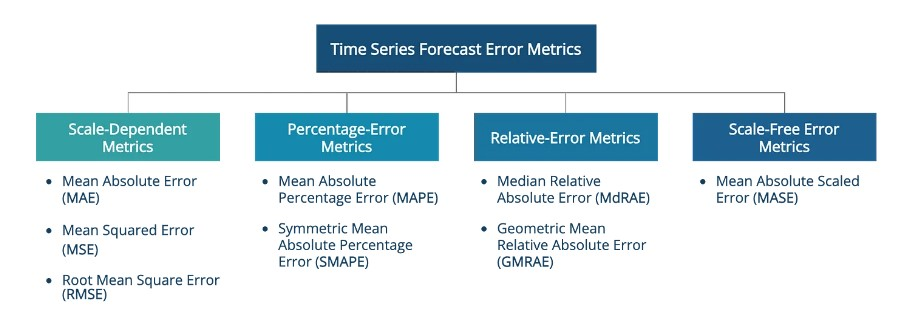
\includegraphics{Tipos_errores_clasificacion_imagen.jpg}

\hypertarget{scale-dependent-metrics}{%
\subsubsection{Scale Dependent Metrics}\label{scale-dependent-metrics}}

Many popular metrics are referred to as scale-dependent (Hyndman, 2006).
Scale-dependent means the error metrics are expressed in the units
(i.e.~Dollars, Inches, etc.) of the underlying data.

The main advantage of scale dependent metrics is that they are usually
easy to calculate and interpret. However, they can not be used to
compare different series, because of their scale dependency (Hyndman,
2006).

Please note here that Hyndman (2006) includes Mean Squared Error into a
scale-dependent group (claiming that the error is ``on the same scale as
the data''). However, Mean Squared Error has a dimension of the squared
scale/unit. To bring MSE to the data's unit we need to take the square
root which leads to another metric, the RMSE. (Shcherbakov et al., 2013)

\hypertarget{mean-absolute-error-mae}{%
\paragraph{Mean Absolute Error (MAE)}\label{mean-absolute-error-mae}}

The Mean Absolute Error (MAE) is calculated by taking the mean of the
absolute differences between the actual values (also called y) and the
predicted values (y\_hat).

Avantages: It is easy to understand (even for business users) and to
compute. It is recommended for assessing accuracy on a single series
(Hyndman, 2006). Disadvantaes: However if you want to compare different
series (with different units) it is not suitable. Also you should not
use it if you want to penalize outliers.

\[MAE = \frac{1}{N}\sum_{1}^{n}\left |e_{t}  \right |=\sum_{1}^{n}\left |yi-\hat{yi} \right|\]

\hypertarget{mean-squared-error-mse}{%
\paragraph{Mean Squared Error (MSE)}\label{mean-squared-error-mse}}

To put more attention on outliers (huge errors) you can consider the
Mean Squared Error (MSE). Like it's name implies it takes the mean of
the squared errors (differences between y and y\_hat).

Due to its squaring, it heavily weights large errors more than small
ones, which can be in some situations a disadvantage. Therefore the MSE
is suitable for situations where you really want to focus on large
errors.

Due to its squaring the metric loses its unit.

Many algorithms (specially ML algorithms) use MSE as it is faster to
compute and easier to manipulate than RMSE. But it is not scaled to the
original error (as the error is squared), resulting in a KPI that we
cannot relate to the original demand scale. Therefore, we won't use it
to evaluate our statistical forecast models.

\[ MSE = \frac{1}{N}\sum_{1}^{n}\left (e_{t})^2  \right|=\sum_{1}^{n}\left (yi-\hat{yi} \right)^2 \]
RMSE emphasizes the most significant errors, whereas MAE gives the same
importance to each error.

\hypertarget{root-mean-squared-error-rmse}{%
\paragraph{Root Mean Squared Error
(RMSE)}\label{root-mean-squared-error-rmse}}

To avoid the MSE's loss of its unit we can take the square root of it.
The outcome is then a new error metric called the Root Mean Squared
Error (RMSE).

It comes with the same advantages as its siblings MAE and MSE. However,
like MSE, it is also sensitive to outliers.

Some authors like Willmott and Matsuura (2005) argue that the RMSE is an
inappropriate and misinterpreted measure of an average error and
recommend MAE over RMSE.

However, Chai and Drexler (2014) partially refuted their arguments and
recommend RMSE over MAE for your model optimization as well as for
evaluating different models where the error distribution is expected to
be Gaussian.

\[ RMSE = {\sqrt{\frac{1}{N}\sum_{1}^{n}\left (e_{t})^2  \right|}} =\sqrt{\sum_{1}^{n}\left (yi-\hat{yi} \right)^2}\]

\hypertarget{percentage-error-metrics}{%
\subsubsection{Percentage Error
Metrics}\label{percentage-error-metrics}}

As we know from the previous chapter, scale dependent metrics are not
suitable for comparing different time series.

Advantage: Percentage Error Metrics solve this problem. They are scale
independent and used to compare forecast performance between different
time series. Disadvantage: Their weak spots are zero values in a time
series. Then they become infinite or undefined which makes them not
interpretable (Hyndman 2006).

\hypertarget{mean-absolute-percentage-error-mape}{%
\paragraph{Mean Absolute Percentage Error
(MAPE)}\label{mean-absolute-percentage-error-mape}}

The mean absolute percentage error (MAPE) is one of the most popular
used error metrics in time series forecasting. It is calculated by
taking the average (mean) of the absolute difference between actuals and
predicted values divided by the actuals.

MAPE's advantages are it's scale-independency and easy interpretability.
As said at the beginning, percentage error metrics can be used to
compare the outcome of multiple time series models with different
scales.

However, MAPE also comes with some disadvantages. First, it generates
infinite or undefined values for zero or close-to-zero actual values
(Kim and Kim 2016).

Second, it also puts a heavier penalty on negative than on positive
errors which leads to an asymmetry (Hyndman 2014).

MAPE have problems on large errors when y-values are close to zero and
the large difference between the absolute percentage errors when y is
greater than y-hat and vice versa.

And last but not least, MAPE can not be used when using percentages make
no sense. This is for example the case when measuring temperatures. The
units Fahrenheit or Celsius scales have relatively arbitrary zero
points, and it makes no sense to talk about percentages (Hyndman and
Koehler, 2006).

\[ MAPE = \frac{1}{N}\sum_{1}^{n}\left (\frac{yi-\hat yi }{yi} \right)*100  \]

\hypertarget{symmetric-mean-absolute-percentage-error-smape}{%
\paragraph{Symmetric Mean Absolute Percentage Error
(sMAPE)}\label{symmetric-mean-absolute-percentage-error-smape}}

The sAMPE is the average across all forecasts made for a given horizon.
It's advantages are that it avoids MAPE's problem of large errors when
y-values are close to zero and the large difference between the absolute
percentage errors when y is greater than y-hat and vice versa. Unlike
MAPE which has no limits, it fluctuates between 0\% and 200\%
(Makridakis and Hibon, 2000).

\[ sMAPE = \frac{1}{N}\sum_{1}^{n}\left(\frac{|yi-\hat yi |}{|yi|+\hat |yi|/2} \right) \]

\hypertarget{mae-vs-rmse}{%
\subsubsection{MAE VS RMSE}\label{mae-vs-rmse}}

\hypertarget{rmse-optimization}{%
\paragraph{RMSE ``optimization''}\label{rmse-optimization}}

Let's take some time to understand why a forecast of the median will get
a good MAE and a forecast of the mean a good RMSE

\url{https://towardsdatascience.com/forecast-kpi-rmse-mae-mape-bias-cdc5703d242d}

To simplify the following algebra, let's use a simplified version: the
Mean Squared Error (MSE):

\[ MSE = \frac{1}{N}\sum_{1}^{n}\left (e_{t})^2  \right|=\sum_{1}^{n}\left (yi-\hat{yi} \right)^2 \]
If you set MSE as a target for your forecast model, it will minimize it.
One can minimize a mathematical function by setting its derivative to
zero. Let's try this.

\begin{Shaded}
\begin{Highlighting}[]
\NormalTok{knitr}\SpecialCharTok{::}\FunctionTok{include\_graphics}\NormalTok{(}\StringTok{"Derivada\_de\_error\_MSE.jpg"}\NormalTok{)}
\end{Highlighting}
\end{Shaded}

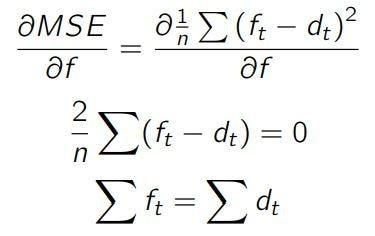
\includegraphics{Derivada_de_error_MSE.jpg}

Conclusion to optimize a forecast's MSE, the model will have to aim for
the total forecast to be equal to the total demand. That is to say that
optimizing MSE aims to produce a prediction that is correct on average
and, therefore, unbiased.

\hypertarget{mae-optimization}{%
\paragraph{MAE ``optimization''}\label{mae-optimization}}

\begin{Shaded}
\begin{Highlighting}[]
\NormalTok{knitr}\SpecialCharTok{::}\FunctionTok{include\_graphics}\NormalTok{(}\StringTok{"Derivada\_error\_MAE\_parte1.jpg"}\NormalTok{)}
\end{Highlighting}
\end{Shaded}

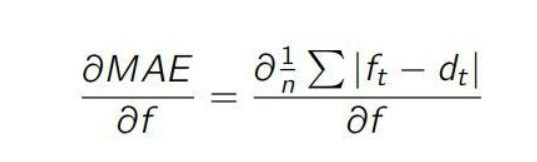
\includegraphics{Derivada_error_MAE_parte1.jpg}

or

\begin{Shaded}
\begin{Highlighting}[]
\NormalTok{knitr}\SpecialCharTok{::}\FunctionTok{include\_graphics}\NormalTok{(}\StringTok{"Derivada\_error\_MAE\_parte2.jpg"}\NormalTok{)}
\end{Highlighting}
\end{Shaded}

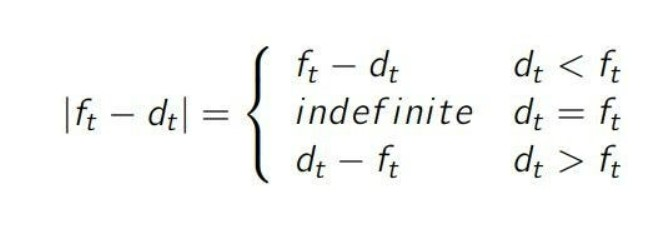
\includegraphics{Derivada_error_MAE_parte2.jpg}

and

\begin{Shaded}
\begin{Highlighting}[]
\NormalTok{knitr}\SpecialCharTok{::}\FunctionTok{include\_graphics}\NormalTok{(}\StringTok{"Derivada\_error\_MAE\_parte3.jpg"}\NormalTok{)}
\end{Highlighting}
\end{Shaded}

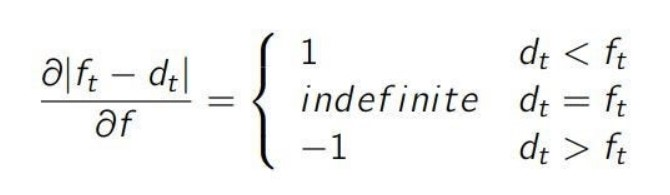
\includegraphics{Derivada_error_MAE_parte3.jpg}

which means:

\begin{Shaded}
\begin{Highlighting}[]
\NormalTok{knitr}\SpecialCharTok{::}\FunctionTok{include\_graphics}\NormalTok{(}\StringTok{"Derivada\_error\_MAE\_parte4.jpg"}\NormalTok{)}
\end{Highlighting}
\end{Shaded}

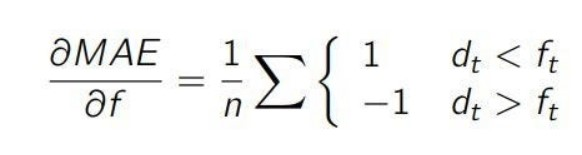
\includegraphics{Derivada_error_MAE_parte4.jpg}

Conclusion to optimize MAE (i.e., set its derivative to 0), the forecast
needs to be as many times higher than the demand as it is lower than the
demand. In other words, we are looking for a value that splits our
dataset into two equal parts. This is the exact definition of the
median.

Let's take some time to discuss the impact of choosing either RMSE or
MAE on bias, sensitivity to outliers, and intermittent demand.

\hypertarget{bias}{%
\paragraph{BIAS}\label{bias}}

For many products, you will observe that the median is not the same as
the average demand. The demand will most likely have some peaks here and
there that will result in a skewed distribution. These skewed demand
distributions are widespread in supply chains as the peaks can be due to
periodic promotions or clients ordering in bulk. This will cause the
demand median to be below the average demand, as shown below.

\begin{Shaded}
\begin{Highlighting}[]
\NormalTok{knitr}\SpecialCharTok{::}\FunctionTok{include\_graphics}\NormalTok{(}\StringTok{"median\_vs\_mean\_left\_skewed\_variable.jpg"}\NormalTok{)}
\end{Highlighting}
\end{Shaded}

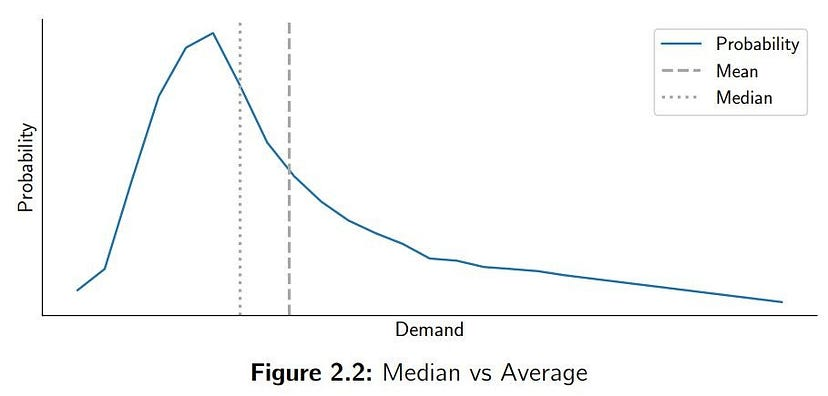
\includegraphics{median_vs_mean_left_skewed_variable.jpg}

This means that a forecast that is minimizing MAE will result in a bias.
In comparison, a forecast minimizing RMSE will not result in bias (as it
aims for the average). This is definitely MAE's main weakness.

\hypertarget{sensitivity-to-outliers}{%
\paragraph{Sensitivity to outliers}\label{sensitivity-to-outliers}}

As we discussed, RMSE gives greater importance to the highest errors.
This comes at a cost: a sensitivity to outliers. Let's imagine an item
with the following demand pattern

Generally speaking, the median is more robust to outliers than the
average. This is rather important in a supply chain environment as we
can face many outliers due to encoding mistakes or demand peaks
(marketing, promotions, spot deals).

\hypertarget{ejemplo-de-calculo-de-varios-tipos-de-errores-para-el-dos-casos-de-suavizamient}{%
\subsubsection{Ejemplo de calculo de varios tipos de errores para el dos
casos de
suavizamient}\label{ejemplo-de-calculo-de-varios-tipos-de-errores-para-el-dos-casos-de-suavizamient}}

Ahora implementemos la función gof que nos permitirá calcular ``muchos
tipos de errores'' entre dos vectores de datos dados
(\url{https://www.youtube.com/watch?v=WBbOh-Z1dmE})

\hypertarget{electrico_demanded_reported-vs-ma_m3_center_placeholder}{%
\paragraph{electrico\_demanded\_reported vs
MA\_M3\_center\_placeholder}\label{electrico_demanded_reported-vs-ma_m3_center_placeholder}}

Tipos de errores entre electrico\_demanded\_reported vs
MA\_M3\_center\_placeholder

\begin{Shaded}
\begin{Highlighting}[]
\FunctionTok{gof}\NormalTok{(}\AttributeTok{sim=}\NormalTok{MA\_m3\_center\_placeholder, }\AttributeTok{obs=}\NormalTok{electrico\_demanded\_reported)}
\end{Highlighting}
\end{Shaded}

\begin{verbatim}
##             [,1]
## ME          0.13
## MAE        72.59
## MSE     12332.85
## RMSE      111.05
## NRMSE %    16.50
## PBIAS %     0.00
## RSR         0.16
## rSD         0.97
## NSE         0.97
## mNSE        0.86
## rNSE        0.98
## d           0.99
## md          0.93
## rd          0.99
## cp          0.77
## r           0.99
## R2          0.97
## bR2         0.97
## KGE         0.97
## VE          0.98
\end{verbatim}

Para calcular el MAPE entre electrico\_demanded\_reported y
MA\_m3\_center\_placeholder

\begin{Shaded}
\begin{Highlighting}[]
\NormalTok{mape\_Reported\_vs\_MA3Center }\OtherTok{\textless{}{-}} \FunctionTok{mean}\NormalTok{(}\FunctionTok{abs}\NormalTok{((electrico\_demanded\_reported }\SpecialCharTok{{-}}\NormalTok{ MA\_m3\_center\_placeholder) }\SpecialCharTok{/}\NormalTok{ electrico\_demanded\_reported), }\AttributeTok{na.rm=}\ConstantTok{TRUE}\NormalTok{) }\SpecialCharTok{*} \DecValTok{100}
\NormalTok{mape\_Reported\_vs\_MA3Center}
\end{Highlighting}
\end{Shaded}

\begin{verbatim}
## [1] 2.287383
\end{verbatim}

En general se nota que ``los pronósticos de MA\_3\_Centrados están
desviados por entre 72-111''puntos'' Lo que respresenta un 2.28\% de
error poercentual

\hypertarget{electrico_demanded_reported-vs-ma_m3_nocenter_placeholder}{%
\paragraph{electrico\_demanded\_reported vs
MA\_M3\_NOcenter\_placeholder}\label{electrico_demanded_reported-vs-ma_m3_nocenter_placeholder}}

Tipos de errores entre electrico\_demanded\_reported vs
MA\_M3\_NOcenter\_placeholder

\begin{Shaded}
\begin{Highlighting}[]
\FunctionTok{gof}\NormalTok{(}\AttributeTok{sim=}\NormalTok{MA\_m3\_NOcenter\_placeholder, }\AttributeTok{obs=}\NormalTok{electrico\_demanded\_reported)}
\end{Highlighting}
\end{Shaded}

\begin{verbatim}
##             [,1]
## ME         -7.65
## MAE       118.91
## MSE     29413.62
## RMSE      171.50
## NRMSE %    25.30
## PBIAS %    -0.30
## RSR         0.25
## rSD         0.98
## NSE         0.94
## mNSE        0.77
## rNSE        0.94
## d           0.98
## md          0.89
## rd          0.99
## cp          0.45
## r           0.97
## R2          0.94
## bR2         0.93
## KGE         0.96
## VE          0.96
\end{verbatim}

Para calcular el MAPE entre electrico\_demanded\_reported y
MA\_m3\_NOcenter\_placeholder

\begin{Shaded}
\begin{Highlighting}[]
\NormalTok{mape\_Reported\_vs\_MA3\_NO\_Center }\OtherTok{\textless{}{-}} \FunctionTok{mean}\NormalTok{(}\FunctionTok{abs}\NormalTok{((electrico\_demanded\_reported }\SpecialCharTok{{-}}\NormalTok{ MA\_m3\_NOcenter\_placeholder) }\SpecialCharTok{/}\NormalTok{ electrico\_demanded\_reported), }\AttributeTok{na.rm=}\ConstantTok{TRUE}\NormalTok{) }\SpecialCharTok{*} \DecValTok{100}
\NormalTok{mape\_Reported\_vs\_MA3\_NO\_Center}
\end{Highlighting}
\end{Shaded}

\begin{verbatim}
## [1] 3.874389
\end{verbatim}

En general se nota que ``los pronósticos de MA\_3\_NO\_Centrados están
desviados por entre 118-171''puntos'' Lo que respresenta un 3.87\% de
error poercentual

\begin{Shaded}
\begin{Highlighting}[]
\NormalTok{knitr}\SpecialCharTok{::}\FunctionTok{include\_graphics}\NormalTok{(}\StringTok{"Check\_list\_for\_selecting\_error\_measure\_depending\_on\_time\_series\_characteristics.jpg"}\NormalTok{)}
\end{Highlighting}
\end{Shaded}

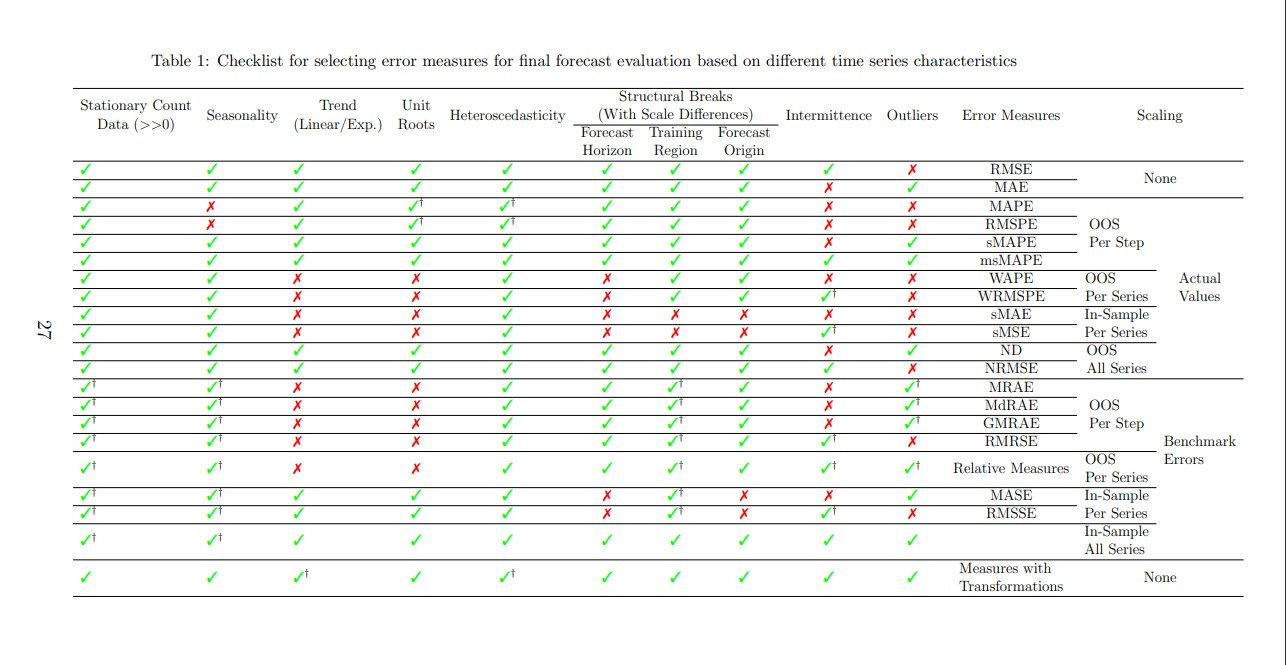
\includegraphics{Check_list_for_selecting_error_measure_depending_on_time_series_characteristics.jpg}

\url{https://arxiv.org/pdf/2203.10716.pdf}

For example, measures with squared base errors such as MSE and RMSE
optimise for the mean whereas others with absolute value base errors
such as MAE and Mean Absolute Scaled Error (MASE) optimise for the
median. Although the mean and median are the same for a symmetric
distribution, that does not hold for skewed distributions as with
intermittent series. There exist numerous controversies in the
literature regarding this. Petropoulos et al.~(2020) suggest that it is
not appropriate to evaluate the same forecastsusing many different error
measures, since each one optimises for a different statistics of the
distribution

Kolassa (2020) further argues that, if the ultimate evaluation measure
is, e.g., MAE which focusses on the median of the distribution, it does
not make sense to optimise the models using an error measure like MSE
(which accounts for the mean). It is more meaningful to consider MAE
also during model training as well.

\end{document}
